\section*{Introduction}

PBPhys is a C library providing structures and functions to simulate system of moving particles in any dimension.\\ 

Each particle is represented by a Shapoid, with a speed and acceleration vector, a mass and a drag coefficient. Particles can be fixed. The PBPhys is defined as GSet of particles. The system can emulate or ignore attraction between particles, downward gravity (applied to the second component of vectors, to simulate earth attraction for example), drag force on particle, elastic collision between particles (considered as perfect spheres). The user can control the system's particle by position, speed or acceleration. The user can step the system by increment of time or until the next collision. The whole system and individual particles can be printed on a stream, saved/loaded in a file.\\

It uses the \begin{ttfamily}PBErr\end{ttfamily}, \begin{ttfamily}PBMath\end{ttfamily}, \begin{ttfamily}Shapoid\end{ttfamily} and \begin{ttfamily}GSet\end{ttfamily} libraries.\\

\section{Definitions}

\subsection{Equation of movement}

The movement of each particle is calculated as follow. Given $drag$ the drag coefficient of the particle ($drag\in\mathbb{R}^+$, 0.0 means no drag), $\overrightarrow{P}(t)$ the position of the particle at instant $t$, $\overrightarrow{S}(t)$ the speed of the particle at instant $t$ and $\overrightarrow{A}(t)$ the acceleration of the particle at instant $t$:\\
\begin{equation}
\overrightarrow{P}(t+\delta t)=\overrightarrow{P}(t)+\overrightarrow{S}(t)\delta t+0.5*(\overrightarrow{A}(t)-drag*\overrightarrow{S}(t))\delta t^2
\end{equation}
\begin{equation}
\overrightarrow{S}(t+\delta t)=\overrightarrow{S}(t)+(\overrightarrow{A}(t)-drag*\overrightarrow{S}(t))\delta t
\end{equation}

If a "downward gravity" is applied, its value is substracted to the second component of the acceleration. If "gravity" is applied each particle $P_i$ 's acceleration is added an attraction force toward others particles equals to:\\
\begin{equation}
\overrightarrow{F}_i(t)=\sum_j\left(G.\frac{m_i.m_j}{||\overrightarrow{P}_j(t)-\overrightarrow{P}_i(t)||^2}.\frac{\overrightarrow{P_j}-\overrightarrow{P_i}}{||\overrightarrow{P}_j(t)-\overrightarrow{P}_i(t)||}\right)
\end{equation} 
where $G$ is the gravity and $m_i$ is the mass of the particle $P_i$.

\subsection{Detection of collision}

The detection of collision between particles is done while approximating particles to spheres.\\

The distance between two particles moving linearly is calculated as follow. Given $\overrightarrow{P}_0(t)$ and $\overrightarrow{S}_0(t)$ the position and speed of the first particle at time $t$, and $\overrightarrow{P}_1(t)$ and $\overrightarrow{S}_1(t)$ the position and speed of the second particle at time $t$. The distance $D(t)$ betwen the two particles is given by:\\
\begin{equation}
D(t_0+dt)=\sqrt{||\overrightarrow{V}(t_0)||^2+2(\overrightarrow{V}(t_0).\overrightarrow{W}(t_0))dt+||\overrightarrow{W}(t_0)||^2dt^2}
\end{equation}
where $\overrightarrow{V}(t)=\overrightarrow{P}_1(t)-\overrightarrow{P}_0(t)$ and $\overrightarrow{W}(t)=\overrightarrow{S}_1(t)-\overrightarrow{S}_0(t)$.\\

One can notice that the square of the distance between particles is a polynomial function of order 2. The time to smallest distance between particles $dt_n$ can then simply be calculated by searching the solution of $D'(t)=0$, which gives:\\
\begin{equation}
dt_n=\frac{-b}{2a}
\end{equation}
where $a$, $b$, $c$ represents the coefficients of the polynomial: $D(t)=at^2+bt+c$.\\

Finally, given $R_0$ and $R_1$ the radius of the spheres approximating the particle, the time $dt_h$ to hit can be calculated as follow:\\
\begin{equation}
dt_h=\frac{-b-\sqrt{b^2-4a(c-(R_0+R_1)^2)}}{2a}
\end{equation}

\subsection{Elastic collision}

The speed after collision of two colliding particles is calculated as follow. Given $m_0$ and $m_1$ the masses of the particles, $\overrightarrow{P}_0$ and $\overrightarrow{P}_1$ the position of the particles, $\overrightarrow{S}_0$ and $\overrightarrow{S}_1$ the speed of the particles before collision and $\overrightarrow{S'}_0$ and $\overrightarrow{S'}_1$ the speed of the particles after collision:\\
\begin{equation}
\overrightarrow{S'}_0=\overrightarrow{S}_0-\frac{2m_1}{m_0+m_1}.\frac{(\overrightarrow{S}_0-\overrightarrow{S}_1).(\overrightarrow{P}_0-\overrightarrow{P}_1)}{||\overrightarrow{P}_0-\overrightarrow{P}_1||^2}(\overrightarrow{P}_0-\overrightarrow{P}_1)
\end{equation}
\begin{equation}
\overrightarrow{S'}_1=\overrightarrow{S}_1-\frac{2m_0}{m_0+m_1}.\frac{(\overrightarrow{S}_1-\overrightarrow{S}_0).(\overrightarrow{P}_1-\overrightarrow{P}_0)}{||\overrightarrow{P}_1-\overrightarrow{P}_0||^2}(\overrightarrow{P}_1-\overrightarrow{P}_0)
\end{equation}

\section{Interface}

\begin{scriptsize}
\begin{ttfamily}
\verbatiminput{/home/bayashi/GitHub/PBPhys/pbphys.h}
\end{ttfamily}
\end{scriptsize}

\section{Code}

\subsection{pbphys.c}

\begin{scriptsize}
\begin{ttfamily}
\verbatiminput{/home/bayashi/GitHub/PBPhys/pbphys.c}
\end{ttfamily}
\end{scriptsize}

\subsection{pbphys-inline.c}

\begin{scriptsize}
\begin{ttfamily}
\verbatiminput{/home/bayashi/GitHub/PBPhys/pbphys-inline.c}
\end{ttfamily}
\end{scriptsize}

\section{Makefile}

\begin{scriptsize}
\begin{ttfamily}
\verbatiminput{/home/bayashi/GitHub/PBPhys/Makefile}
\end{ttfamily}
\end{scriptsize}

\section{Unit tests}

\begin{scriptsize}
\begin{ttfamily}
\verbatiminput{/home/bayashi/GitHub/PBPhys/main.c}
\end{ttfamily}
\end{scriptsize}

\section{Unit tests output}

\begin{scriptsize}
\begin{ttfamily}
\verbatiminput{/home/bayashi/GitHub/PBPhys/unitTestRef.txt}
\end{ttfamily}
\end{scriptsize}

traj.txt:\\
\begin{scriptsize}
\begin{ttfamily}
\verbatiminput{/home/bayashi/GitHub/PBPhys/traj.txt}
\end{ttfamily}
\end{scriptsize}
\begin{center}
\begin{figure}[H]
\centering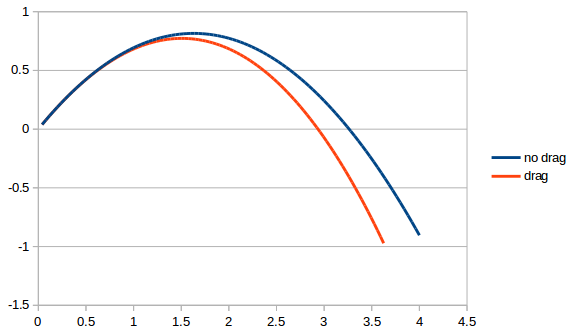
\includegraphics[width=10cm]{./trajectory.png}\\
\end{figure}
\end{center}

collision.txt:\\
\begin{scriptsize}
\begin{ttfamily}
\verbatiminput{/home/bayashi/GitHub/PBPhys/collision.txt}
\end{ttfamily}
\end{scriptsize}
\begin{center}
\begin{figure}[H]
\centering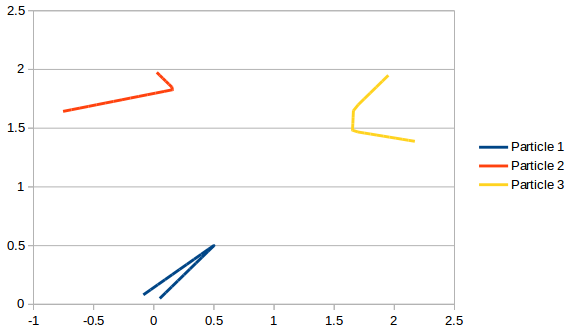
\includegraphics[width=10cm]{./collision.png}\\
\end{figure}
\end{center}


